\documentclass[11pt,letterpaper]{article}
\usepackage[lmargin=1in,rmargin=1in,tmargin=1in,bmargin=1in]{geometry}
\usepackage{../style/homework}
\usepackage{../style/commands}
\setbool{quotetype}{true} % True: Side; False: Under
\setbool{hideans}{false} % Student: True; Instructor: False

% -------------------
% Content
% -------------------
\begin{document}

\homework{7: Due 03/03}{Today is a good day to try.}{Quasimodo, The Hunchback \par of Notre Dame}

% Problem 1
\problem{10} Being as accurate as possible, sketch the graph of the line $2x - 3y= 12$.
	\[
	\fbox{
	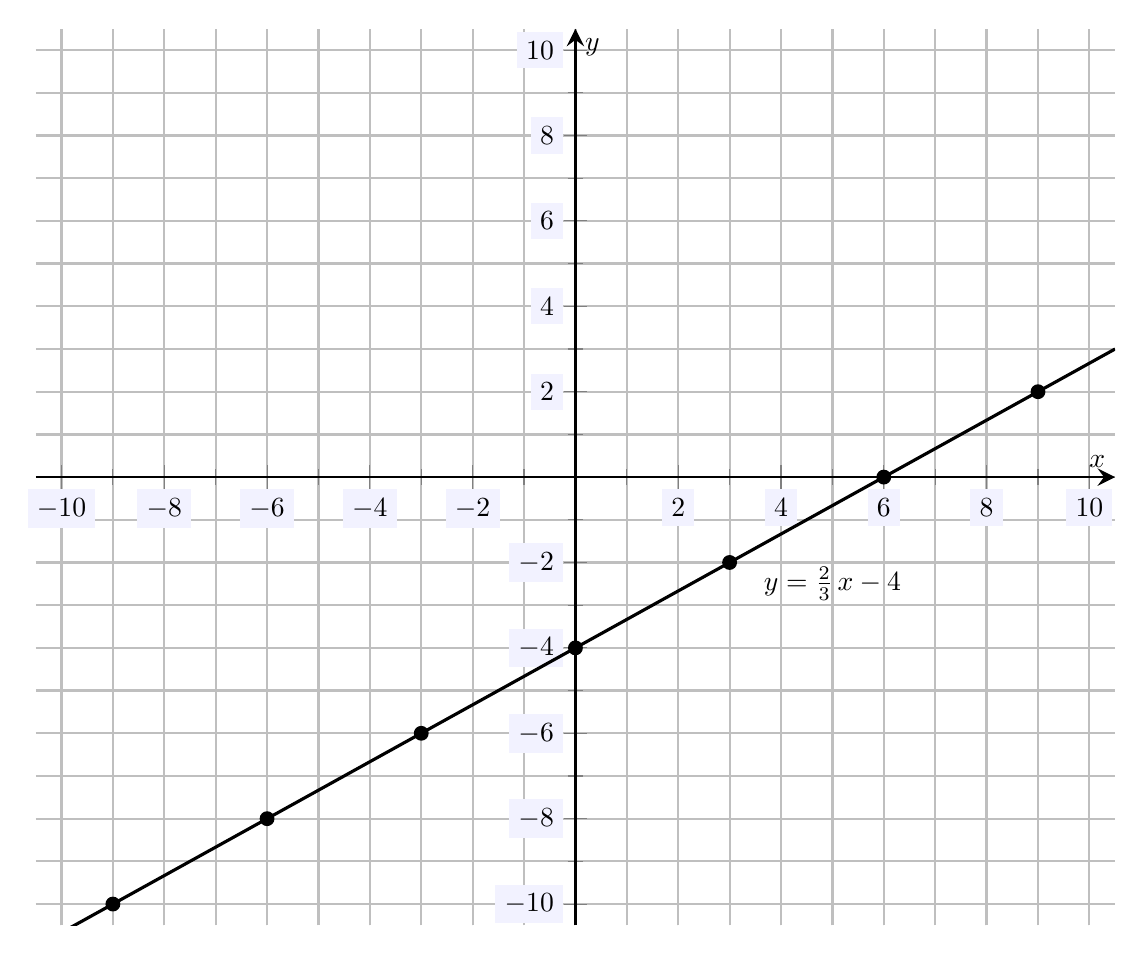
\begin{tikzpicture}[scale=2,every node/.style={scale=0.5}]
	\begin{axis}[
	grid=both,
	axis lines=middle,
	ticklabel style={fill=blue!5!white},
	xmin= -10.5, xmax=10.5,
	ymin= -10.5, ymax=10.5,
	xtick={-10,-8,-6,-4,-2,0,2,4,6,8,10},
	ytick={-10,-8,-6,-4,-2,0,2,4,6,8,10},
	minor tick = {-10,-9,...,10},
	xlabel=\(x\),ylabel=\(y\),
	]
	\draw[fill=black] (-9,-10) circle (0.04cm);
	\draw[fill=black] (-6,-8) circle (0.04cm);
	\draw[fill=black] (-3,-6) circle (0.04cm);
	\draw[fill=black] (0,-4) circle (0.04cm);
	\draw[fill=black] (3,-2) circle (0.04cm);
	\draw[fill=black] (6,0) circle (0.04cm);
	\draw[fill=black] (9,2) circle (0.04cm);
	\node at (5.0,-2.5) {$y= \frac{2}{3}\,x - 4$};
	\addplot[line width= 0.02cm,domain= -10.5:10.5] ({x},{2/3*x - 4}); 
	\end{axis}
	\end{tikzpicture}
	}
	\] \pspace

We can solve for $y$ in the equation $2x - 3y= 12$:
	\[
	\begin{aligned}
	2x - 3y&= 12 \\
	-3y&= -2x + 12 \\
	y&= \frac{2}{3}\,x - 4
	\end{aligned}
	\]
This line has slope $m= \frac{2}{3}$ and $y$-intercept $b= -4$ (technically, $(0, -4)$). We can then use the `slope' method of plotting: interpreting the slope $m= \frac{2}{3}$ as $\frac{\Delta y}{\Delta x}$, we see that for each increase of 3 in $x$ results in an increase of 2 in $y$. Alternatively, writing $m= \frac{2}{3}= \frac{-2}{-3}$, each decrease of 3 in $x$ results in a decrease of 2 in $y$. Using this, we can create a series of points to smoothly connect in the plot above. 



\newpage



% Problem 2
\problem{10} Consider the linear function $f(x)= 5 - \frac{3}{4}\,x$.
	\begin{enumerate}[(a)]
	\item Find the slope of this linear function. 
	\item Interpret the slope two different ways.
	\item Is the linear function increasing, decreasing, or constant? Explain. 
	\item Determine the $y$-intercept for $f(x)$.
	\item Determine the $x$-intercept for $f(x)$.
	\end{enumerate} \pspace

\sol
\begin{enumerate}[(a)]
\item Because this is a linear function, it must be able to be put in the form $y= mx + b$, where $m$ is the slope. Here, we have $y= f(x)$, $x= x$, $m= -\frac{3}{4}$, and $b= 5$. Therefore, the slope is $m= -\frac{3}{4}$. \pspace

\item Interpreting the slope $m= -\frac{3}{4}= \frac{-3}{4}$ as $\frac{\Delta y}{\Delta x}$, we see that for every increase of 4 in $x$, there is a corresponding decrease of 3 in $y$. Alternatively, writing $m= -\frac{3}{4}= \frac{3}{-4}$, we see that for every decrease of 4 in $x$, we see a corresponding increase of 3 in $y$. Finally, another `immediate' interpretation is given by writing $m= -\frac{3}{4}= -0.75= \frac{-0.75}{1}$. Then for every increase of 1 in $x$, we see a corresponding decrease of 0.75 in $y$. Alternatively, writing $m= -\frac{3}{4}= -0.75= \frac{0.75}{-1}$. Then for every decrease of 1 in $x$, we see a corresponding increase of 0.75 in $y$. \pspace

\item Because $m= -\frac{3}{4} < 0$, we see that this linear function is decreasing in $x$. \pspace

\item Because this is a linear function, it must be able to be put in the form $y= mx + b$, where $b$ is the $y$-intercept (technically, $(0, b)$). Here, we have $y= f(x)$, $x= x$, $m= -\frac{3}{4}$, and $b= 5$. Therefore, the $y$-intercept is $b= 5$---technically, $(0, 5)$. \pspace

\item The $x$-intercept occurs when $f(x)$ passes through the $x$-axis, i.e. when the output is 0. But then $f(x)= 0$. We can then solve for $x$:
	\[
	\begin{aligned}
	f(x)&= 0 \\
	5 - \frac{3}{4}\,x&= 0 \\
	\frac{3}{4}\,x&= 5 \\
	\frac{4}{3} \cdot \frac{3}{4}\,x&= 5 \cdot \frac{4}{3} \\
	x&= \frac{20}{3}
	\end{aligned}
	\]
Therefore, the $x$-intercept is $\frac{20}{3}$---technically, $(\frac{20}{3}, 0)$. 
\end{enumerate}



\newpage



% Problem 3
\problem{10} Showing all your work, find the equation of the line perpendicular to $y= 5 - 3x$ that passes through the point $(1, -4)$. \pspace

\sol Because the line is perpendicular to the line $y= 5 - 3x$---which is `sloped', we know that the line is not vertical. Therefore, the line must have the form $y= mx + b$. Because the line is perpendicular to the line $y= 5 - 3x$, the slope of the line must be the negative reciprocal of the slope of the line $y= 5 - 3x$. The slope of the line $y= 5 - 3x$ is $-3$. The negative reciprocal of this is $-(\frac{1}{-3})= \frac{1}{3}$. Therefore, we have $m= \frac{1}{3}$ so that $y= \frac{1}{3}x + b$. But we know that the line passes through the point $(1, -4)$, i.e. when $x= 1$, we know $y= -4$. But then\dots
	\[
	\begin{aligned}
	y&= \frac{1}{3}\,x + b \\
	-4&= \frac{1}{3} \cdot 1 + b \\
	-4&= \frac{1}{3} + b \\
	b&= -4 - \frac{1}{3} \\
	b&= -\frac{12}{3} - \frac{1}{3} \\
	b&= -\frac{13}{3}
	\end{aligned}
	\]
Therefore, the equation of the line is $y= \frac{1}{3}x - \frac{13}{3}$. \pspace
	\[
	\boxed{%
	y= \frac{1}{3}x - \frac{13}{3}
	}
	\]



\newpage



% Problem 4
\problem{10} Showing all your work, solve the following linear equation, be sure to verify that your solution satisfies the equation: 
	\[
	5x - 6= 1 - 7x
	\] \pspace

\sol 
	\[
	\begin{aligned}
	5x - 6&= 1 - 7x \\[0.3cm]
	12x - 6&= 1 \\[0.3cm]
	12x&= 7 \\[0.3cm]
	x&= \dfrac{7}{12}
	\end{aligned}
	\] \pspace

We can check this solution: \pspace
	\[
	\begin{aligned}
	5x - 6&= 1 - 7x \\[0.3cm]
	5 \cdot \dfrac{7}{12} - 6&\stackrel{?}{=} 1 - 7 \dfrac{7}{12} \\[0.3cm]
	\dfrac{35}{12} - 6&\stackrel{?}{=} 1 - \dfrac{49}{12} \\[0.3cm]
	\dfrac{35}{12} - \dfrac{72}{12}&\stackrel{?}{=} \frac{12}{12} - \dfrac{49}{12} \\[0.3cm]
	-\frac{37}{12}&= -\frac{37}{12} \\
	&\,\,\text{\cmark}
	\end{aligned}
	\] \pspace



\newpage



% Problem 5
\problem{10} Water is flowing into a `rectangular' box with side lengths 2~ft, 4~ft, and 5~ft at a rate of 3.4~ft$^3$/min. Currently, the box contains 16~ft$^3$ of water. Let $W(t)$ denote the amount of water in the box $t$ minutes from now.
	\begin{enumerate}[(a)]
	\item Explain why $W(t)$ is linear.
	\item Find $W(t)$. 
	\item What do the slope and $y$-intercept of $W(t)$ represent in context?
	\item Determine when the box will begin to overflow. 
	\end{enumerate} \pspace

\sol
\begin{enumerate}[(a)]
\item The water is flowing into the container at a constant rate. Because the rate of change is constant, we know that $W(t)$ must be linear. \pspace

\item Clearly, $W(t)$ is not a vertical line. Therefore, $W(t)$ must have the form $W(t)= mt + b$. We know at time $t= 0$ that the box contains 16~ft$^3$ of water. But then $16= W(0)= m(0) + b= 0 + b= b$ so that $b= 0$. We know also that the water is flowing into the box at a rate of 3.4~ft$^3$ per minute. But then we know that $m= 3.4$ so that $W(t)= 3.4t + 16$. \pspace

\item We have $W(t)= 3.4t + 16$. The slope is $m= 3.4$, which is the rate of flow of water into the box. The $y$-intercept is 16 (properly, $(0, 16)$), which corresponds to the fact that at the `start' (the initial time) the box contains 16~ft$^3$ of water. \pspace

\item The box has volume $V= \ell w h= 2 \cdot 4 \cdot 5= 40$~ft$^3$. The box will overflow once the amount of water, $W(t)$, is 40~ft$^3$. But then we have\dots
	\[
	\begin{aligned}
	W(t)&= 40 \\
	3.4t + 16&= 40 \\
	3.4t&= 24 \\
	t&= 7.059 \text{ min}
	\end{aligned}
	\]
Therefore, the box will begin to overflow after 7.059~minutes, i.e. 7 minutes and 3.54~seconds.
\end{enumerate}


\end{document}